\documentclass[11pt]{article}
\usepackage[includeheadfoot, top=1.0in, bottom=1.0in, hmargin=1.0in]{geometry}
\usepackage[utf8]{inputenc}
\usepackage{fancyhdr}
\pagestyle{fancy}
\usepackage{setspace}
\usepackage{tabularx}
\usepackage{xcolor}
\usepackage{cancel}
\usepackage{amsmath,amsfonts}
\usepackage{graphicx}
\usepackage{siunitx}
\usepackage{amssymb}

\usepackage[hyphens]{url}
\usepackage{hyperref}
\usepackage{enumitem}

\lhead{Astronomy Lab II}
\rhead{Spring 2023}
\lfoot{Golant}
\rfoot{Tue 7-10pm}
\cfoot{\thepage}

\begin{document}

\begin{center}
\huge{Lab 4: Stars \& Stellar Evolution}\\ \medskip \Large{February 14, 2023}
\end{center}

\section{Introduction: Reaching for the Stars}

\section{Building an H-R Diagram}
Before looking at any data or making any plots, let's make some hypotheses. \textbf{Record your responses in your lab write-up}:
\begin{enumerate}
    \item \textcolor{blue}{4 pts} What trends (if any) do you expect to emerge when we plot a group of stars on a brightness vs. temperature plot? Beyond just brightness and temperature, think about how stellar mass, size, color, and chemical makeup might affect a star's position on the plot.
    
    \item \textcolor{blue}{4 pts} How do you expect the H-R diagram to change when we plot brightness vs. \emph{color} instead of brightness vs. temperature? (hint: stars can be well-approximated as black bodies!) 
    
\end{enumerate}

\subsection{The brightest stars}
% explain magnitude, luminosity, color. how are mag and luminosity related to brightness?

Open up the spreadsheet named ``stars.xlsx'' in the ``Lab 4'' folder under the ``Files'' tab on CourseWorks. The first tab of the spreadsheet (labeled ``brightest'') contains data for the 34 brightest stars in the night sky. Using this data, \textbf{complete the following, recording your responses in your lab write-up}:
\begin{enumerate}
    \setcounter{enumi}{2}
    
    \item An H-R diagram plots \emph{brightness} vs. \emph{surface temperature} (i.e., the temperature of the outer layer of a star). However, there are multiple ways of quantifying brightness. The \textbf{luminosity} expresses the intrinsic energy output of a star -- effectively, how much light is produced per second. On the other hand, the \textbf{magnitude}, a unitless quantity, expresses brightness on an inverse logarithmic scale (where, confusingly, \emph{smaller} or \emph{more negative} magnitudes correspond to \emph{brighter} stars).
    \begin{enumerate}
        \item \textcolor{blue}{3 pts} Construct an H-R diagram for these 34 bright stars by making a scatter plot with the logarithm of \emph{luminosity} (see column ``log(Luminosity)'' on the spreadsheet) on the vertical axis and the surface temperature on the horizontal axis. For historical reasons, the temperature should \emph{increase} as we move to the \emph{left} along the diagram, so make sure to \emph{invert} your horizontal axis. Make sure your axes are labeled with the correct units!

    \begin{figure}[h!]
        \centering
        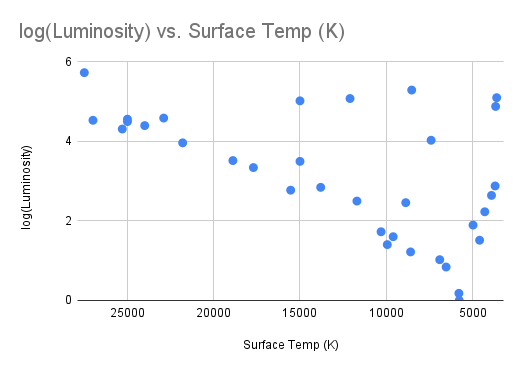
\includegraphics[width=0.5\textwidth]{Images/luminosity - brightest.png}
        \label{fig:my_label}
    \end{figure}
        
        \item \textcolor{blue}{3 pts} Now, construct an H-R diagram with the \emph{absolute magnitude} on the vertical axis (and, again, surface temperature on the horizontal axis). Since we want brightness to \emph{increase} up the vertical axis, use the ``Absolute Magnitude (V-band) Reverse y-axis'' column on the spreadsheet, which should place lower magnitudes \emph{above} higher magnitudes. Again, make sure to invert your horizontal axis.

    \begin{figure}[h!]
        \centering
        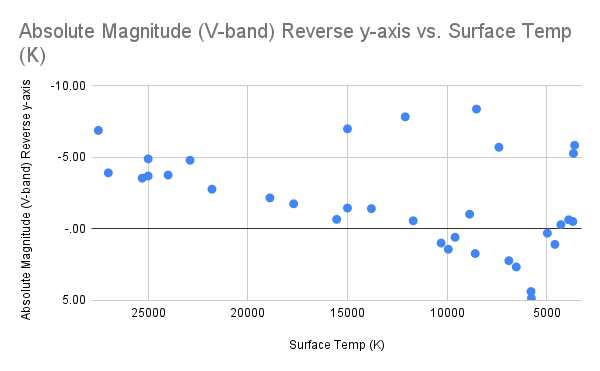
\includegraphics[width=0.5\textwidth]{Images/mag - brightest.png}
        \label{fig:my_label}
    \end{figure}
        
        \item \textcolor{blue}{3 pts} What differences (if any) do you notice between these two H-R diagrams? For most of this lab, we'll be working with magnitudes rather than luminosities, since the magnitude scale is more popular amongst observational astronomers.

        \textcolor{red}{The most luminous, hottest star lies above the red giants in the luminosity plot, but below in the magnitude plot - the scaling is different between the two, representative of how we convert to magnitudes.}
    \end{enumerate}
    
    \item \textcolor{blue}{4 pts} On your magnitude vs. temperature H-R diagram from above, do you see any groups or clumps of stars? If so, describe where on the diagram these groups lie, and (if possible) circle or box these groups on your diagram.
    \textcolor{red}{Grade based on reasoning.  Ideally they recognize the MS and red giants.}
    
    \item \textcolor{blue}{3 pts} Where does the Sun lie on your diagram? Compared to the rest of the stars, is the Sun brighter or dimmer than average? Is the Sun hotter or colder than average?
    \textcolor{red}{Sun lies low on plot, low log luminosity and low temperature.}
    
    \item \textcolor{blue}{4 pts} The stars populating the upper-right corner of your diagram are very bright but relatively cold. How can a star put out such a large amount of light while having such a low temperature?
    \textcolor{red}{Very massive, but cold.}
    
    \item \textcolor{blue}{4 pts} Do you think the H-R diagram you've plotted for these bright stars is representative of all stars? Why or why not?
    \textcolor{red}{Grade based on reasoning. These are selectively the brightest stars in the sky, which could be affected by distance and intrinsic brightness. This does not include dim stars, even if near.}
    
\end{enumerate}

\subsection{The closest stars}
Now, go to the second tab in ``stars.xlsx,'' labeled ``nearest.'' This sheet contains data for the 30 closest stars to Earth. \textbf{Complete the following in your lab write-up}:
\begin{enumerate}
\setcounter{enumi}{7}

    \item \textbf{Before looking at any new plots}, consider the \emph{biases} in the two data sets we've considered so far (i.e., the brightest stars and the closest stars). Whenever you're working with any data set (astronomical or otherwise), it's imperative that you always consider how the data may be biased!
    \begin{enumerate}
        \item \textcolor{blue}{4 pts} Do you expect your H-R diagram of the closest stars to differ from your H-R diagram of the brightest stars? Why and how?
        \textcolor{red}{Grade based on reasoning. The closest stars are not selectively brightest and should have a range of properties. So should differ from the brightest stars.}
        
        \item \textcolor{blue}{4 pts} Do you expect your H-R diagram of the closest stars to differ from that of the general population of stars? Why and how?
        \textcolor{red}{Grade based on reasoning.  No, there is no reason that the stars nearby should differ statistically from the general population. There is nothing special about this region of the galaxy.}
    \end{enumerate}
    
    \item \textcolor{blue}{3 pts} Now, construct an H-R diagram for the 30 closest stars by again making a scatter plot with the (reversed) magnitude on the vertical axis and the surface temperature on the horizontal axis. Once again, remember to invert your horizontal axis so that temperature is greatest to the \emph{left} of the diagram.

    \begin{figure}[h!]
        \centering
        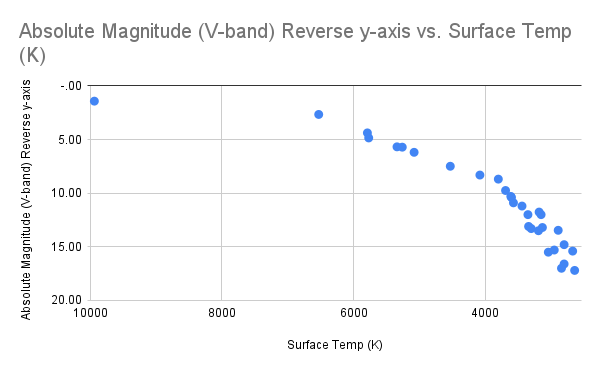
\includegraphics[width=0.5\textwidth]{Images/mag - nearest.png}
        \label{fig:my_label}
    \end{figure}
    
    \item \textcolor{blue}{3 pts} How does your H-R diagram for the closest stars differ from your H-R diagram for the brightest stars?
    \textcolor{red}{We get dimmer stars}
    
    \item \textcolor{blue}{3 pts} How does the Sun compare to other nearby stars (in terms of, for example, brightness and temperature)?
    \textcolor{red}{Fairly average}
    
\end{enumerate}

\subsection{The full diagram}
You should have seen a slight difference between your two H-R diagrams, with the diagram of the brightest stars having more points towards the top right and top left of the plot, while the diagram of the nearest stars should have had more points closer to the Sun and towards the bottom right of the diagram. Now, let's combine these two populations onto a single diagram. \textbf{Complete the following in your lab write-up}:
\begin{enumerate}
\setcounter{enumi}{11}

    \item \textcolor{blue}{3 pts} Go to the ``combined'' tab on the ``stars.xlsx'' spreadsheet and once again make a scatter plot of magnitude vs. surface temperature.

    \begin{figure}[h!]
        \centering
        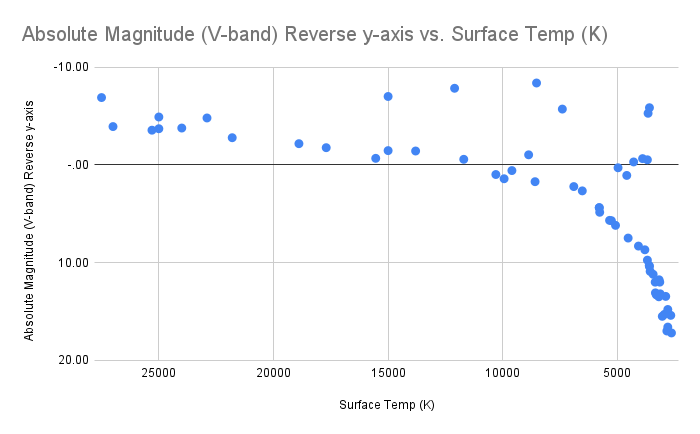
\includegraphics[width=0.5\textwidth]{Images/mag - combine.png}
        \label{fig:my_label}
    \end{figure}
    
    \item Stars spend most of their lives on the so-called \emph{main sequence}. Main-sequence stars span a wide range of magnitudes and temperatures.
    \begin{enumerate}
        \item \textcolor{blue}{3 pts} Where is the main sequence on your H-R diagram? 
         \textcolor{red}{Primary line of stars (some stars lie above)}
        
        \item \textcolor{blue}{3 pts} Not all stars lie on the main sequence -- \emph{giant} stars are brighter and (on average) cooler than main sequence stars. Where is the giant branch on your H-R diagram?
        \textcolor{red}{upper right corner}
        
        \item \textcolor{blue}{7 pts} Given the position of the giant branch relative to the main sequence, propose a hypothesis as to how giant stars and main sequence stars may be connected. What evidence (i.e., data and observations) would support your hypothesis?
        \textcolor{red}{Grade based on reasoning.}
    
    \end{enumerate}
    
    \item We're still missing a key component of the H-R diagram: the \emph{white dwarfs}.
    \begin{enumerate}
        \item \textcolor{blue}{3 pts} Using data from the ``complete'' tab of the ``stars.xlsx'' spreadsheet, plot an H-R diagram complete with a main sequence, a giant branch, and a population of white dwarfs.

    \begin{figure}[h!]
        \centering
        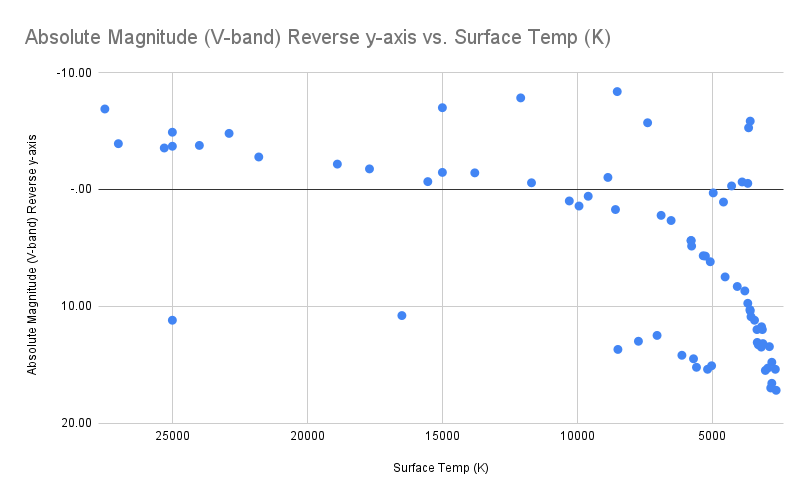
\includegraphics[width=0.5\textwidth]{Images/mag - complete.png}
        \label{fig:my_label}
    \end{figure}
        
        \item Compare your new diagram to your previous diagrams to help identify the white dwarfs.
        \begin{enumerate}
            \item \textcolor{blue}{3 pts} Describe, roughly, where the white dwarfs are located on the H-R diagram. 
            \textcolor{red}{lower left corner}
            
            \item \textcolor{blue}{4 pts} In terms of brightness and surface temperature, how do white dwarfs compare to main sequence stars?
            \textcolor{red}{They are hotter but less luminous than MS stars.}
        \end{enumerate}
        
        \item \textcolor{blue}{7 pts} Where do you think white dwarfs come from? That is, how do you think we end up with this rogue population of stars in this region of the H-R diagram? What evidence would support your hypothesis?
        \textcolor{red}{Grade based on reasoning.}
    \end{enumerate}
    
    
    % need to make sure we only plot main sequence%
    \item \textcolor{blue}{10 pts} Your friend tells you that the mass of main sequence stars \emph{increases} as you move upwards and towards the left along the main sequence. Use the data provided to dispute or support this claim. (the data on the ``main sequence'' tab of ``stars.xlsx'' may be helpful)
    \textcolor{red}{Grade based on reasoning.}
     
    
\end{enumerate} 

\section{Stellar Evolution}
We've already talked a little about how the structure of the H-R diagram hints at the underlying process of stellar evolution. Now, let's see this in action. Navigate to \url{https://starinabox.lco.global/}; this ``Star in a Box'' applet animates stellar evolution along the H-R diagram. Click ``Open the Lid'' to see the H-R diagram. Use this applet to \textbf{answer the following questions in your lab write-up}:
\begin{enumerate}
\setcounter{enumi}{15}

    \item \textcolor{blue}{3 pts} Using the drop-down menu in the bottom left corner, progressively vary the initial mass of the star from 0.2 solar masses to 40 solar masses. The black dot on the H-R diagram denotes the star's initial position on the main sequence. How does varying the mass change the star's position along the main sequence? Is this consistent with what you saw in the previous section?
    \textcolor{red}{With increasing mass, the MS position moves from lower right to upper left.}
    
    \item For each mass, click the play button (the right-arrow in the lower right corner of the applet) to watch the star evolve; if the animation is too fast, you can adjust the animation speed with the drop-down menu to the right of the play button.
    \begin{enumerate}
    
        \item \textcolor{blue}{7 pts} Describe the evolution of a Sun-like star (i.e., a star with an initial mass of 1 solar mass) in the context of the H-R diagram. What do you think is happening to the star as it traverses the nearly-horizontal stretch towards the top of its evolutionary track? (hint: for a fixed luminosity, a star's radius and temperature vary inversely)
        \textcolor{red}{Grade based on reasoning. The Sun remains on the MS for a long time, then becomes a red giant.  Finally it becomes a white dwarf.  The horizontal track is when the Sun becomes a white dwarf.  The luminosity is fixed, but the temperature rapidly increases, so the radius of the star must be rapidly decreasing.}
        
        \item \textcolor{blue}{10 pts} In the previous section, you discovered the main sequence, the giant branch, and the white dwarfs by plotting a collection of stars on the H-R diagram. How are these three populations connected via stellar evolution?
        \textcolor{red}{Stars are born on the MS.  When they start burning helium, they become red giants. When they are no longer able to do nuclear fusion, they become white dwarfs.}
        
        \item \textcolor{blue}{6 pts} By varying the initial mass, you should find that there are three possible ways in which a star can complete its life. What are these three end-of-life scenarios (or, rather, what are the three possible end products)? At roughly which \emph{initial} stellar masses do we transition from one end product to another?
        \textcolor{red}{White Dwarf $<10 M_\odot$, Neutron Star 10 $< M_* <$ 30 $M_\odot$, Black Hole $> 30 M_\odot$}
        
    \end{enumerate}
    
    \item \textcolor{blue}{0 pts} By clicking on ``Data Table'' in the upper-right corner of the applet, you can find detailed information about a star at each stage of its life. This data table varies for each initial mass. 
    \begin{enumerate}
        \item As you increase the initial mass, how does the amount of time a star spends on the main sequence change?
        \textcolor{red}{The time on the MS decreases as mass increases.}
        
        \item A star leaves the main sequence once it's used up all the hydrogen fuel in its core. A star's luminosity quantifies how quickly the star burns up its fuel. Given what you know about the relationship between mass and luminosity along the main sequence, explain why the trend you found in the previous question makes sense.
        \textcolor{red}{The more massive stars are brighter and so use their H more quickly.  Since they only burn H on the MS, they leave the MS more quickly.}
        
        \item You're trying to learn about a cluster of stars that you just discovered in the far reaches of the Milky Way. So, you decide to plot an H-R diagram of the stars contained in the cluster. You notice that your H-R diagram contains a large number of blue giants, or stars near the upper-left of the main sequence. What does this tell you about the age of the star cluster?
        \textcolor{red}{The massive stars are still on the MS, meaning the cluster has to be very young.}
        
    \end{enumerate}
\end{enumerate}



\section{Wrapping Things Up}
\textbf{Answer the following questions in your lab write-up}:
\begin{enumerate}
\setcounter{enumi}{18}

    \item Reflect a bit on the H-R diagram:
    \begin{enumerate}
        \item \textcolor{blue}{4 pts} In a sentence, describe what an H-R diagram is.
        \textcolor{red}{The H-R diagram plots the temperature and luminosity of all stars and can be used to understand stellar evolution.}
        
        \item\textcolor{blue}{4 pts} Describe the major groups of stars that show up on an H-R diagram. 
        \textcolor{red}{MS - stars doing hydrogen fusion, Giants - stars after MS, WD - low mass end of life scenario (stellar core)}
        \begin{enumerate}
            \item How do the properties of a typical star in each of these groups compare to those of our Sun?
            \textcolor{red}{MS - about the same, Giants - more luminous but cooler, WD - dimmer, hotter}
        \end{enumerate} 
        
        \item \textcolor{blue}{4 pts} Describe briefly how the process of stellar evolution connects to the H-R diagram.
        \textcolor{red}{Stars are born on the MS. They do H-fusion, then become giant stars and move off the MS. They then undergo 1 of 3 EoL scenarios - for low mass stars, we are left with the cooling stellar core, which sits in the bottom left of the plot.}
        
    \end{enumerate}
    
    
    \item \textcolor{blue}{0 pts} The Vogt-Russell theorem states that the mass and chemical composition of a star \emph{completely} determine the evolutionary trajectory of a star, from birth to death. 
    \begin{enumerate}
        \item Explain how the Vogt-Russell theorem motivates the H-R diagram. That is, how does the Vogt-Russell theorem make the H-R diagram ``useful?''
        
        \item If the Vogt-Russell theorem didn't hold, could we still use the H-R diagram to predict the life cycle of a star?
    \end{enumerate}
    
    \item On the Ed Discussion page, post at least one question that you still have after finishing this lab.
    
    \item If you have any feedback on how today's lab was run, or if you have any suggestions for future lab sessions, please let me know!
    
    
\end{enumerate}


\end{document}